%% Evaluation section

\section{Evaluation}
\label{sec:evaluation}
To rigorously assess the performance of \approach{}, we evaluate four research questions:

\begin{itemize}
	\item \textbf{RQ1 (Effectiveness)}: How does \approach{} perform relative to state-of-the-art methods in terms of precision and recall?
	\item \textbf{RQ2 (Ablation Study)}: To what extent do the RAG engine and two-stage retrieval mechanism contribute to the system's diagnostic capability?
	\item \textbf{RQ3 (Efficiency and Cost)}: What are the operational latencies and computational overheads of \approach{}?
	\item \textbf{RQ4 (Capability Boundaries)}: In which categories of exploits does \approach{} excel or falter?
\end{itemize}

These RQs are motivated as follows. \textbf{RQ1} validates whether retrieval-augmented reasoning translates into tangible detection gains over representative learning-based and analysis-based baselines. \textbf{RQ2} isolates the contributions of knowledge injection (RAG) and retrieval refinement, clarifying which component is responsible for the observed improvements. \textbf{RQ3} characterizes the end-to-end latency and API cost footprint, which ultimately determines whether \approach{} is viable for near-real-time deployment. \textbf{RQ4} identifies systematic strengths and failure modes across attack categories, delineating the practical capability boundary and guiding future extensions.

% \subsection{Experimental Setup}

\textit{\textbf{Benchmark.}}
We evaluate \approach{} on two datasets with complementary goals: \textit{\dsystem{}} for broad-spectrum detection and \textit{\done{}} for price manipulation. \dsystem{} contains 728 transactions with a balanced 1:1 ratio between malicious and benign samples (364 each): malicious transactions were curated from publicly documented incidents in DeFiHackLabs~\cite{defihacklabs2024} (Jan.~2021--Jan.~2025; 110+ exploit types across Ethereum/BSC/Arbitrum), while benign transactions were collected from the same protocols and filtered by temporal proximity; Table~\ref{tab:attack_categories} summarizes the category distribution. \done{} is the public dataset released with DeFiScope~\cite{zhong2025detectingvariousdefiprice} (95 real-world price manipulation cases; \$381.16M total loss); using our trace collection pipeline, we retrieved complete call-flow data for 91 transactions used in the experiments.

\begin{table}[t]
	\caption{Attack Category Distribution in \dsystem{} Dataset}
	\label{tab:attack_categories}
	\centering
	%\small
	\setlength{\tabcolsep}{4pt}
	\begin{tabular}{lrr}
		\toprule
		\textbf{Attack Category} & \textbf{Count} & \textbf{\%} \\
		\midrule
		Business Logic Flaws & 125 & 34.3 \\
		Price-related Attacks & 65 & 17.9 \\
		Reentrancy \& Call Attacks & 43 & 11.8 \\
		Access Control Vulnerabilities & 31 & 8.5 \\
		Input Validation Issues & 22 & 6.0 \\
		Flashloan-driven Attacks & 22 & 6.0 \\
		Mathematical Calculation Issues & 19 & 5.2 \\
		Token Mechanism Vulnerabilities & 10 & 2.7 \\
		Other (20+ subtypes) & 27 & 7.4 \\
		\midrule
		\textbf{Total} & \textbf{364} & \textbf{100.0} \\
		\bottomrule
	\end{tabular}
\end{table}



\textit{\textbf{Baselines.}}
We benchmark \approach{} against strong baselines aligned with each dataset: on \dsystem{}, TrxGNNBERT~\cite{TrxGNNBERT} (a Graph-Transformer model for transaction graphs); on \done{}, DeFiScope~\cite{zhong2025detectingvariousdefiprice} (pattern learning), DeFort~\cite{defort2024} (symbolic execution), DeFiRanger~\cite{defiranger2021} (state-change analysis), and DeFiTainter~\cite{defitainter2023} (dynamic taint tracking).
Together, these baselines cover learning-based, formal, and dynamic analysis paradigms for a balanced comparison.


\textit{\textbf{Experiment Setup.}}
To ensure consistent inference conditions across heterogeneous models, all large language models used in our experiments were accessed through third-party API providers. \approach{} is implemented using LangChain~\cite{langchain} with Chroma~\cite{chromadb} as the vector database. Unless otherwise specified, we use GPT-4.1-mini as the primary reasoning engine and Jina Embeddings v3~\cite{jina2024} to generate vector representations. To prevent data leakage, we construct the knowledge base from a randomly sampled set of 210 DeFiHackLabs historical attack incidents, disjoint from the evaluated attack transactions. The retrieval stage (vector search + filtering) completes in under 100~ms; end-to-end latency is dominated by LLM inference, averaging 15~seconds with GPT-4.1-mini and as low as 11.82~seconds with Llama-3.1-8B-Instruct. We report Accuracy, Precision, Recall, F1-score, and average end-to-end processing latency.

% \textit{\textbf{Compute Environment and API Access.}}
% % Due to limited local GPU resources, 
% To ensure consistent inference conditions across heterogeneous models, all large language models used in our experiments were accessed through third-party API providers. All evaluations used identical prompting configurations without model‑specific tuning, and token and latency measurements therefore reflect real‑world deployment behavior rather than controlled offline execution.



% \textit{\textbf{System Implementation.}}
% \approach{} is implemented using LangChain~\cite{langchain} with Chroma~\cite{chromadb} as the vector database. Unless otherwise specified, we use GPT-4.1-mini as the primary reasoning engine. We use Jina Embeddings v3~\cite{jina2024} to generate vector representations. To prevent data leakage, we construct the knowledge base from a randomly sampled set of 210 DeFiHackLabs historical attack incidents spanning April 2018 to December 2020, which is disjoint from the evaluated attack transactions; the retrieval stage (vector search + filtering) completes in under 100~ms. End-to-end latency is dominated by LLM inference, averaging 15~seconds with GPT-4.1-mini and as low as 11.82~seconds with Llama-3.1-8B-Instruct.

% \textit{\textbf{Evaluation Metrics.}}
% We report Accuracy, Precision, Recall, F1-score, and average end-to-end processing latency.

\subsection{RQ1 (Effectiveness): Comparative Analysis of Detection Accuracy}
To provide a comprehensive assessment of \approach{}'s detection efficacy, we conducted comparative experiments across two datasets with distinct characteristics.

\textit{\textbf{Overall effectiveness and latency.}}
As detailed in \Cref{tab:performance-dsystem-compact}, when configured with GPT-4.1-mini as its reasoning engine, \approach{} achieves an F1-score of 0.839, with precision and recall reaching 0.832 and 0.846, respectively, and an overall accuracy of 0.838. This performance consistently outperforms all evaluated baselines, including the state-of-the-art TrxGNNBERT (F1: 0.766), Blockscan (F1: 0.810), and Txspector (F1: 0.533). Notably, while Blockscan attains a very high precision (0.955), its recall is significantly lower (0.701), indicating a conservative detection strategy that tends to mislabel novel or complex attacks as benign. In contrast, \approach{} strikes a superior balance between precision and recall, delivering the highest F1 score and overall accuracy among all compared methods. Furthermore, Txspector suffers from inherent limitations in its rule-based EVM tracing engine, resulting in low recall (0.571), incomplete transaction coverage (only 450 out of 728 transactions), and an impractical processing latency of several hours. Beyond detection accuracy, \approach{} demonstrates a decisive edge in efficiency; its average processing latency is approximately 15~seconds, which is $20\times$ faster than TrxGNNBERT ($\sim$5~minutes) and orders of magnitude faster than Txspector's manual rule-based pipeline, making it suitable for near-real-time deployment.

% \begin{table}[H]
% 	\centering
% 	\caption{Performance Comparison on the \dsystem{} Dataset}
% 	\label{tab:performance-dsystem-compact}
% 	%\small
% 	\begin{tabular}{lccccc}
% 		\toprule
% 		\textbf{Tool} & \textbf{Accuracy} & \textbf{Precision} & \textbf{Recall} & \textbf{F1-Score} & \textbf{Avg. Latency} \\
% 		\midrule
% 		TrxGNNBERT & 0.759 & 0.760 & 0.773 & 0.766 & $\sim$5 min \\
% 		%\approach{}(Ours) & 0.822 & 0.782 & 0.894 & 0.834 & 15.02 s \\
% 		\approach{}(Ours) & 0.812 & 0.774 & 0.882 & 0.824 & 15.02 s \\
% 		\bottomrule
% 	\end{tabular}
% \end{table}


\begin{table}[t]
	\centering
	\caption{Performance Comparison on the \dsystem{} Dataset}
	\label{tab:performance-dsystem-compact}
	%\small
	\begin{tabular}{lccccc}
		\toprule
		\text{Tool} & \text{Accuracy} & \text{Precision} & \text{Recall} & \text{F1-Score} & \text{Avg. Latency} \\
		\midrule
		Txspector \cite{zhang2020txspector} & 0.544 & 0.500 & 0.571 & 0.533 & $\sim$hours \\
		TrxGNNBERT \cite{TrxGNNBERT} & 0.759 & 0.760 & 0.773 & 0.766 & $\sim$5 min \\
		Blockscan\cite{wu2025blockscan} & 0.834 & 0.955 & 0.701 & 0.810 & 25 s \\
		\approach{}(Ours) & \textbf{0.838} & \textbf{0.832} & \textbf{0.846} & \textbf{0.839} & 15.02 s \\
		\bottomrule
	\end{tabular}
\end{table}


\textit{\textbf{Sensitivity to the LLM backbone.}}
Building upon these results, we further investigated how different large language models influence \approach{}, as summarized in \Cref{tab:ragflow_results}. The Llama-3.1-8B-Instruct variant achieved the lowest processing latency of 11.82~seconds while maintaining a competitive F1-score of 0.793, demonstrating an excellent balance between efficiency and accuracy. Similarly, the ERNIE-Speed-128k model offered a favorable trade-off with a latency of 12.66~seconds and an F1-score of 0.809. Meanwhile, the GPT-4.1-mini variant yielded the highest accuracy metrics across the board (F1: 0.839), validating the synergistic effect between high-performance language models and the RAG framework.

\begin{figure}[t]
	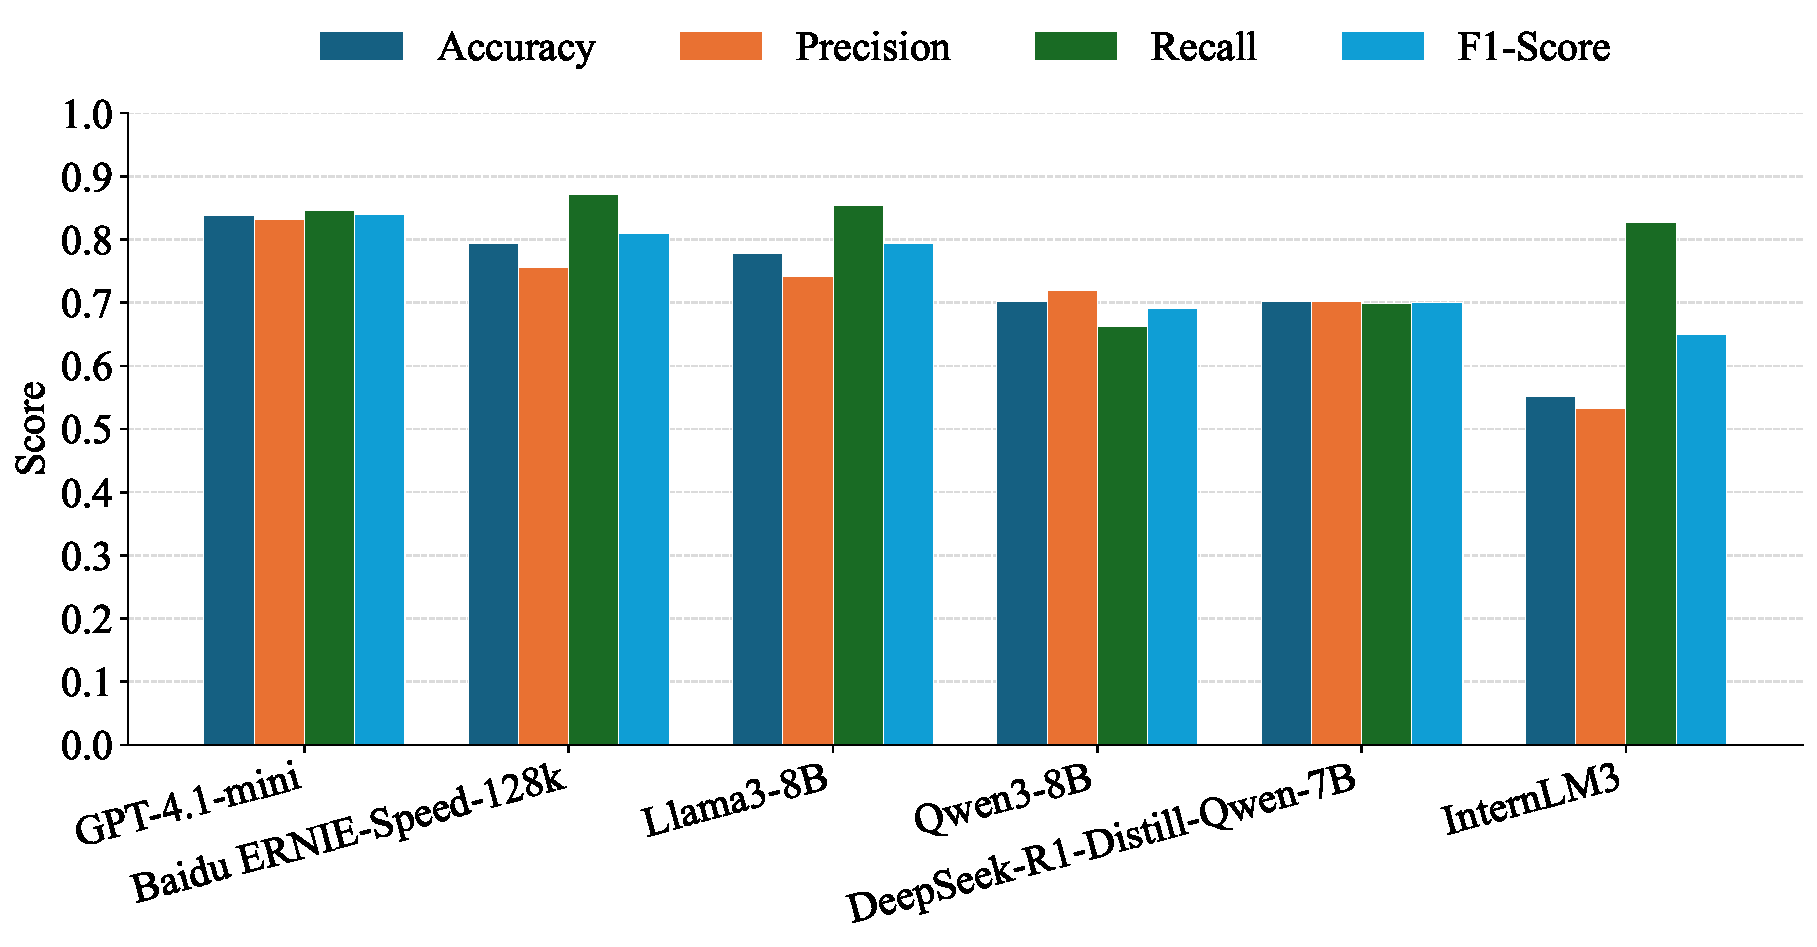
\includegraphics[width=.8\linewidth]{pic/model_performance_column_chart.pdf}
	\caption{Performance Comparison across Different Models on the \dsystem{} Dataset}
	\label{tab:ragflow_results}
\end{figure}

% \begin{table*}[htbp]
% 	\centering
% 	\caption{Performance of \approach{} with Different Models on the \dsystem{} Dataset}
% 	\label{tab:ragflow_results}
% 	\begin{tabular}{lccccr}
% 		\toprule
% 		Model & Accuracy & Precision & Recall & F1-Score & Avg. Latency (s) \\
% 		\midrule
% 		% GPT-4.1-mini & 0.812 & 0.774 & 0.882 & 0.824 & 15.02 \\
%         GPT-4.1-mini & 0.838 & 0.832 & 0.846 & 0.839 & 15.02 \\
% 		Baidu ERNIE-Speed-128k & 0.794 & 0.755 & 0.871 & 0.809 & 12.66 \\
% 		Llama3-8B & 0.778 & 0.741 & 0.854 & 0.793 & 11.82 \\
% 		Qwen3-8B & 0.702 & 0.719 & 0.662 & 0.690 & 37.54 \\
% 		DeepSeek-R1-Distill-Qwen-7B & 0.702 & 0.702 & 0.698 & 0.700 & 32.31 \\
% 		InternLM3 & 0.551 & 0.533 & 0.827 & 0.649 & 12.70 \\
% 		\bottomrule
% 	\end{tabular}
% \end{table*}

\textit{\textbf{Price manipulation recall.}}
Driven by the high criticality of price manipulation attacks, we performed a specialized evaluation using the public dataset \done{}. As shown in Table~\ref{tab:recall-d1-dataset}, the GPT-3.5-turbo-backed version of \approach{} achieved a recall of 95.60\%, significantly outperforming the best-performing baseline, DeFiScope (80.22\%). This performance gap stems from a fundamental methodological divergence: while traditional tools like DeFiRanger and DeFort rely on precise mathematical modeling of specific pricing functions, \approach{} emphasizes semantic reasoning grounded by retrieved historical patterns, enabling it to better handle non-standard or custom pricing logic.

\begin{table}[htbp]
	\centering
	\caption{Recall Comparison on \done{} Dataset (91 Price Manipulation Cases)}
	\label{tab:recall-d1-dataset}
	%\setlength{\tabcolsep}{4pt} % 缩小列间距（关键）
	\begin{tabular}{l c c c}
		\toprule
		\text{Tool} &
		\text{\#Attack} &
		\text{Recall} &
		\text{$\Delta$Recall (w.r.t. DeFiScope)} \\
		\midrule
		\approach{} (GPT-3.5-turbo) & 87  & 95.60\% & +15.38\% \\
		\approach{} (GPT-4.1-mini)  & 86 & 94.51\% & +14.29\% \\
		DeFiScope (DS)          & 73  & 80.22\% & \textbf{Baseline} \\
		DeFort (DF)             & 50  & 54.95\% & $-$25.27\% \\
		DeFiRanger (DR)         & 48  & 52.75\% & $-$27.47\% \\
		DeFiTainter (DT)        & 32  & 35.16\% & $-$45.06\% \\
		\bottomrule
	\end{tabular}
\end{table}

\textit{\textbf{Error analysis: missed cases.}}
Despite its robust overall performance, \approach{} encountered challenges in a few highly intricate cases. Table~\ref{tab:ragflow_false_negative} provides a granular breakdown of five misclassifications for \approach{} with GPT-4.1-mini. For instance, the IndexedFinance attack involved an index token manipulation mechanism that was not widely recognized at the time, while the BeltFinance series featured complex, multi-step cross-contract interactions. It is worth noting, however, that these cases proved equally challenging for traditional tools; in most instances, at least two baseline tools also failed to provide a correct detection.


\begin{table}[H]
	\centering
	\caption{\approach{}'s Missed Cases and Baseline Tool Detection Results}
	\label{tab:ragflow_false_negative}
	%\small
	\begin{tabular}{l c c c c}
		\toprule
		Attack Case & DS & DT & DF & DR \\
		\midrule
		MerlinLab & \ding{51} & \ding{55} & \ding{55} & \ding{55} \\
		BeltFinance\_1 & \ding{51} & \ding{51} & \ding{55} & \ding{51} \\
		BeltFinance\_2 & \ding{51} & \ding{51} & \ding{55} & \ding{51} \\
		IndexedFinance & \ding{55} & \ding{55} & \ding{55} & \ding{51} \\
		ERC20TokenBank & \ding{51} & \ding{55} & \ding{55} & \ding{51} \\
		\bottomrule
	\end{tabular}
	
	\vspace{0.3em}
	\footnotesize\textit{DS=DeFiScope, DT=DeFiTainter, DF=DeFort, DR=DeFiRanger. \ding{51}=detected, \ding{55}=missed.}
\end{table}


\textit{\textbf{Error analysis: failure modes.}}
A deep dive into these misjudgments reveals that \approach{}’s limitations are primarily confined to four scenarios. First are rare or highly customized oracle manipulation patterns (e.g., MerlinLab), which exploit idiosyncratic oracle update windows; the absence of sufficiently similar historical samples causes analogical reasoning to falter. Second, the system struggles with arbitrage attacks involving complex multi-step cross-contract interactions (e.g., BeltFinance), where attackers leverage minute price discrepancies through sequences of transactions that appear legitimate in isolation, making full-chain reconstruction difficult. Third, novel attacks utilizing innovative mechanisms (e.g., IndexedFinance), such as exploiting index token rebalancing weights, fall outside the scope of historical patterns or rule-based detection. Finally, atypical price manipulation edge cases (e.g., ERC20TokenBank) manipulate internal accounting logic rather than liquidity pool pricing, a paradigm shift that often leads to omissions by most detection tools.


\textit{\textbf{Takeaways.}}
In summary, the effectiveness of \approach{} in DeFi attack detection is anchored in three core strengths: the retrieval-augmented mechanism that leverages domain knowledge for informed reasoning; a semantic-level analysis that transcends the limitations of traditional mathematical modeling; and a modular architecture that balances performance with operational efficiency. Nevertheless, there remains room for improvement in addressing rare attack patterns, complex multi-step exploits, and entirely novel mechanisms. These strengths and constraints collectively delineate the capability boundaries of \approach{} as a competitive and practical solution for DeFi security.

\subsection{RQ2 (Ablation Study): Quantifying the Contributions of Core Components}
%\textit{\textbf{Summary.}}
Table~\ref{tab:ragflow-ablation} shows that retrieval augmentation is the decisive driver of \approach{}’s effectiveness (absolute F1 gain: 0.586), while two-stage retrieval is a secondary optimizer that improves context quality and contributes an additional 0.030 to F1.

\textit{\textbf{Setup.}}
To ascertain the individual contributions of \approach{}’s core modules and justify their architectural inclusion, we performed a series of ablation experiments on the \dsystem{} dataset using GPT-4.1-mini as the LLM backbone. The experimental results are summarized in Table~\ref{tab:ragflow-ablation}.


% \begin{table}[htbp]
% 	\centering
% 	\caption{Ablation Study of \approach{} Core Components on \dsystem{} Dataset}
% 	\label{tab:ragflow-ablation}
% 	\normalsize
% 	\begin{tabular}{lcccc}
% 		\toprule
% 		\multirow{2}{*}{\textbf{Experimental Configuration}} & \multicolumn{4}{c}{\textbf{Performance Metrics}} \\
% 		\cmidrule(lr){2-5}
% 		& \textbf{F1} & \textbf{Prec.} & \textbf{Rec.} & \textbf{Acc.} \\
% 		\midrule
% 		Full \approach{} System & 0.824 & 0.774 & 0.882 & 0.812 \\
% 		w/o Two-Stage Retrieval & 0.794 & 0.743 & 0.852 & 0.779 \\
% 		w/o RAG Framework & 0.238 & 0.785 & 0.140 & 0.551 \\
% 		\bottomrule
% 	\end{tabular}

% 	\smallskip\scriptsize\textit{Note: ``w/o Two-Stage'' disables retrieval refinement; ``w/o RAG'' removes retrieval augmentation.}
% \end{table}

\begin{table}[htbp]
	\centering
	\caption{Ablation Study of \approach{} Core Components on \dsystem{} Dataset}
	\label{tab:ragflow-ablation}
	\normalsize
	\begin{tabular}{lcccc}
		\toprule
		\multirow{2}{*}{\textbf{Experimental Configuration}} & \multicolumn{4}{c}{\textbf{Performance Metrics}} \\
		\cmidrule(lr){2-5}
		& \textbf{F1} & \textbf{Prec.} & \textbf{Rec.} & \textbf{Acc.} \\
		\midrule
		Full \approach{} System & 0.839 & 0.832 & 0.846 & 0.838 \\
		w/o XGBoost & 0.824 & 0.774 & 0.882 & 0.812 \\
		w/o Two-Stage Retrieval & 0.794 & 0.743 & 0.852 & 0.779 \\
		w/o RAG Framework & 0.238 & 0.785 & 0.140 & 0.551 \\
		\bottomrule
	\end{tabular}

	\smallskip\scriptsize\textit{Note: ``w/o XGBoost'' disables the XGBoost post-processor; ``w/o Two-Stage'' disables retrieval refinement; ``w/o RAG'' removes retrieval augmentation entirely.}
\end{table}

\textit{\textbf{Effect of adding the XGBoost post-processor.}}
Incorporating the XGBoost post-processor improves precision from 0.774 to 0.832, a gain of 0.058, while slightly reducing recall from 0.882 to 0.846, a decrease of 0.036. This trade‑off yields a net F1 improvement from 0.824 to 0.839. The precision gain indicates that the XGBoost filter effectively reduces false positives by learning a decision boundary over the LLM’s output features, making the system more suitable for production environments where false alarms are costly. The moderate recall loss is acceptable given the overall F1 improvement and the substantial reduction in false positives.

\textit{\textbf{Effect of removing retrieval augmentation.}}
Disabling retrieval augmentation and relying on a vanilla LLM causes a catastrophic collapse: the F1-score plummets from 0.824 to 0.238, and recall drops from 0.882 to 0.140. This sharp decline highlights a fundamental limitation of general-purpose LLMs in DeFi attack detection, where parametric knowledge alone is often insufficient in both depth and temporal relevance. Injecting structured historical evidence shifts the model from heuristic guessing to evidence-driven reasoning, contributing an absolute F1 gain of 0.586.

\textit{\textbf{Effect of removing two-stage retrieval.}}
Reverting to simple vector retrieval without the second-stage filtering leads to a smaller but consistent performance drop: F1 declines from 0.824 to 0.794. This result indicates that while basic retrieval can recover many relevant cases, the second-stage filtering (dynamic thresholding and contract exclusion) acts as a quality gate that removes low-discriminative documents and mitigates leakage risks, yielding a cleaner context for LLM reasoning and more stable decisions.

\textit{\textbf{Discussion.}}
Taken together, the ablation results quantitatively map the hierarchical contributions of \approach{}’s core components. The RAG framework provides the primary impetus for effectiveness by grounding the LLM with evidence, contributing an absolute F1 gain of 0.586. The two-stage retrieval further refines the context quality, adding a modest 0.030 to the F1 score. Finally, the XGBoost post-processor delivers a precision‑focused enhancement of 0.058, with only a small recall penalty, resulting in a net F1 improvement of 0.015. This layered design demonstrates that combining evidence‑based reasoning, retrieval refinement, and lightweight post‑processing yields a robust and practical detection system.


\subsection{RQ3 (Efficiency): Practical Latency, Cost Analysis, and Deployment Viability}

Having established the detection efficacy and structural integrity of \approach{}, we now pivot to its pragmatic engineering feasibility. In the high-stakes domain of smart contract security, the real-world utility of any monitoring system is strictly governed by its operational latency and resource overhead. To ascertain whether \approach{} can be seamlessly integrated into live threat-detection pipelines, we evaluate its performance across two pivotal dimensions: temporal efficiency and economic sustainability.

\textit{\textbf{Processing Latency.}} As evidenced by the performance metrics in Table~\ref{tab:ragflow_results}, \approach{} demonstrates a promising throughput suitable for near-real-time analysis. The system achieves an average end-to-end latency of 15.02 seconds when utilizing GPT-4.1-mini. This can be further optimized to 11.82 seconds with Llama-3.1-8B-Instruct and 12.66 seconds with Baidu ERNIE-Speed-128k. Such efficiency is largely underpinned by the optimized synergy between the RAG engine and our two-stage retrieval mechanism, a design choice that drastically prunes the search space before Large Language Model (LLM) inference begins. Notably, the retrieval stage itself (vector search followed by filtering) completes in under 100ms. Our profiling reveals that peak latencies are primarily driven by LLM inference cycles and network propagation during API calls, rather than internal computational bottlenecks like vector database queries or context distillation.

\textit{\textbf{Cost-Benefit Analysis.}} We conducted a granular assessment of operational expenditures across both datasets, as detailed in Table~\ref{tab:api_cost_comparison}. For the relatively compact \done{} dataset (91 samples), GPT-4.1-mini consumed approximately 5.43 million tokens at a cumulative cost of \$2.24, whereas GPT-3.5-Turbo required 5.87 million tokens, totaling \$3.15. Scaling the evaluation to the more extensive \dsystem{} dataset (728 samples) unveiled distinct efficiency profiles among the models. While GPT-4.1-mini processed the entire corpus for \$3.86, the Llama-3.1-8B-Instruct model demonstrated the capacity to slash costs to roughly \$0.26, a reduction of over 93\%.



\textit{\textbf{API Utilization and Token Efficiency.}}
To better understand the cost characteristics of different models, we analyzed token consumption during live API evaluation. The results indicate that model-specific verbosity remains a key factor shaping overall token usage. Qwen3-8B produced comparatively longer responses, with outputs reaching up to 29~KB (approximately 7,400 tokens), resulting in a total of 8.15M tokens. InternLM3-8B-Instruct generated more compact outputs, though its total volume (8.2M tokens) remained similar due to retrieval-induced input overhead. DeepSeek-R1-Distill-Qwen-14B exhibited the highest efficiency among the evaluated models, with a total of 7.7M tokens. These observations highlight the combined influence of output verbosity and retrieval context on API-level cost.


\textit{\textbf{Cross-Chain Scalability.}} While our evaluation primarily focuses on Ethereum and BSC, where most attack cases are currently observed, \approach{} is designed to be extendable to other EVM-compatible blockchains, such as Polygon and Arbitrum. This adaptability ensures that the framework remains applicable as malicious activities evolve and expand across different blockchain ecosystems.

\begin{table}[htbp]
	\caption{Estimated API Cost Comparison Across Datasets}
	\label{tab:api_cost_comparison}
	\centering
	%\footnotesize
	%\small
	\renewcommand{\arraystretch}{1}
	\setlength{\tabcolsep}{1pt}
	\begin{tabular}{>{\raggedright}p{0.4\columnwidth}
			>{\centering\arraybackslash}p{0.12\columnwidth}
			>{\centering\arraybackslash}p{0.12\columnwidth}}
		\toprule
		\textbf{Model} & \textbf{Tokens} & \textbf{Cost(\$)} \\
		\midrule
		\multicolumn{3}{l}{\textbf{\done{} (91 samples)}} \\
		\midrule
		GPT-4.1-mini & 5.43M & 2.24 \\
		GPT-3.5-turbo & 5.87M & 3.15 \\
		\midrule
		\multicolumn{3}{l}{\textbf{\dsystem{} (728 samples)}} \\
		\midrule
		GPT-4.1-mini & 8.62M & 3.86 \\
		Llama-3.1-8B-Instruct & 8.28M & 0.26 \\
		Baidu ERNIE-Speed-128k & 11.62M & FREE \\
		InternLM3-8B-Instruct & 8.2M & FREE \\
		DeepSeek-R1-Distill-Qwen-14B & 7.7M & FREE \\
		Qwen3-8B & 8.15M & FREE \\
		\bottomrule
	\end{tabular}
	
	% \vspace{0.3em}
	\smallskip\scriptsize\textit{Note: Costs are estimated from public API rates; token counts are total input+output per query, as reported by the API providers.}
\end{table}


As shown in Table~\ref{tab:api_cost_comparison}, such discrepancies, where output volumes vary by a factor of three for identical retrieval-augmented queries, underscore the critical impact of model selection on a system's economic viability. Crucially, the stable and economical output characteristics of models like InternLM3-8B-Instruct suggest that by prioritizing token efficiency without sacrificing analytical depth, the \approach{} framework can achieve a high degree of financial sustainability. Furthermore, the convergence of low operational cost (\$0.26) and competitive latency (11.82 seconds) positions Llama-3.1-8B-Instruct as a particularly compelling candidate for practical deployment. These empirical findings collectively reinforce the prospect of deploying \approach{} in high-frequency production environments where both precision and cost-efficiency are paramount.

\subsection{RQ4: Capability Boundaries}
To better understand the operational boundaries of \approach{}, we conducted a systematic analysis of its detection performance across the \dsystem{} dataset, specifically examining the interplay between attack mechanisms and technical features. Our findings reveal that \approach{}'s efficacy is distributed across a distinct spectrum, primarily dictated by three core dimensions: the observability of malicious behavior, the analogicality of semantic patterns, and the contextual dependency of the attack logic. This spectrum not only defines the current capability limits of \approach{} but also provides critical insights for its real-world deployment and future iteration. Table~\ref{tab:capability_spectrum} summarizes the detection performance across different attack categories.

\textit{\textbf{Core Dimensions and Definitions.}}
To characterize \approach{}'s capability boundaries, we organize attacks along three dimensions that align with its decision pipeline: (i) \emph{trace-level behavioral evidence}, (ii) \emph{retrieval-based analogy to historical cases}, and (iii) \emph{multi-step/cross-contract context integration}. Specifically, \textit{Observability} measures whether execution traces expose discriminative behavioral deviations (e.g., anomalous external-call/state-update patterns); \textit{Analogicality} measures whether such deviations form reusable semantic templates that can be matched to prior incidents in the knowledge base; \textit{Contextual dependency} measures the extent of global context required to infer intent, especially when signals are distributed across long, multi-step, or cross-contract interactions.
Based on these dimensions, Table~\ref{tab:capability_spectrum} summarizes a capability spectrum: categories dominated by observable and reusable patterns are easier to detect, whereas categories requiring broad context integration or exhibiting behaviorally compliant traces approach the system’s natural boundary.

\textit{\textbf{Definition of Difficulty Levels.}}
We label each category in Table~\ref{tab:capability_spectrum} by the primary bottleneck it presents to \approach{}. \textbf{Low}: high observability and strong analogicality (clear, repetitive trace signatures). \textbf{Medium}: observable core semantics but weaker reusability due to protocol-specific or highly variable logic (analogy-dependent). \textbf{High}: strong contextual dependency, where intent emerges only after aggregating evidence across long, multi-step, or cross-contract execution chains. \textbf{Fundamental}: low observability at the trace-semantic level, where execution remains behaviorally compliant and the malice stems from cryptographic or protocol-assumption violations beyond behavior-only semantics.


\begin{table}[htbp]
	\centering
	\caption{\approach{} Detection Performance by Attack Category}
	\label{tab:capability_spectrum}
	\small
	\begin{tabular}{lcc}
		\toprule
		\textbf{Attack Category} & \textbf{Detection Rate} & \textbf{Difficulty} \\
		\midrule
		Reentrancy & 96.2\% & Low \\
        Price \& Oracle Manipulation & 93.2\% & Low \\
		Flash-loan Price Manipulation & 91.7\% & Low \\
		Business Logic Flaws & 89.6\% & Medium \\
		Liquidity \& Migration Exploits & 87.5\% & Medium \\
		Arbitrary Call / External Call & 86.7\% & Medium \\
		Access Control & 79.3\% & Medium \\
		Fake Market / MEV / Sandwich Attacks & 75.0\% & High \\
		Signature \& Validation Issues & 57.1\% & High \\
		Cryptographic Exploits  & $<$50\% & Fundamental \\
		\bottomrule
	\end{tabular}
	
	\smallskip\scriptsize\textit{Note: Cross-contract reentrancy exploits are merged into Reentrancy due to limited samples (2 cases).}
\end{table}


\textit{\textbf{Dominant Capability (High Observability + High Analogicality).}} \approach{} demonstrates its most resilient detection capabilities in scenarios where behavioral anomalies are highly observable and semantic patterns remain stable and reusable. Typical examples include classic reentrancy exploits (96.2\%), flash-loan price manipulations (91.7\%), and price/oracle manipulations (93.2\%). These attacks generate explicit, identifiable signatures within the execution flow, such as the ``unprivileged call to privileged function'' pattern seen in the LocalTrader series, or the ``unexpected state change following an external call'' characteristic of the SpankChain reentrancy exploit. Because the core malicious semantics of these attacks are highly repetitive, \approach{} can leverage its historical case library to establish a robust mapping between ``symptoms'' and ``attack types.'' Consequently, even when encountering novel variants, the system maintains high detection rates through stable pattern matching.

\textit{\textbf{Competitive Capability (Moderate Observability, Analogy-Dependent).}}
Moving into the domain of common but more sophisticated DeFi exploits---such as Access Control (79.3\%), business logic flaws (89.6\%), arbitrary external calls (86.7\%), liquidity/migration exploits (87.5\%), reflection/token economics flaws, and storage/proxy issues---the system’s performance begins to exhibit fluctuations influenced by the complexity and novelty of the attack patterns. In this domain, \approach{} effectively identifies signatures such as the ``unprivileged call to privileged function'' pattern (e.g., LocalTrader series) or anomalous asset transfer sequences when the knowledge base contains analogous patterns (e.g., Platypus attack). However, performance is challenged by highly innovative or combinatorial variants. For instance, the Indexed Finance exploit utilized a then-novel index token weight rebalancing mechanism; the absence of directly comparable cases in the knowledge base can lead to false negatives. Similarly, variants employing non-standard mechanisms---such as the UwU Lend exploit’s use of median pricing across multiple pools---require the underlying LLM to perform deep reasoning over novel logic rather than simple pattern matching. This area represents a transition for \approach{} from ``pattern matching'' to ``semantic comprehension,'' where accuracy is strictly gated by the breadth of the knowledge base and the model’s reasoning depth.

\textit{\textbf{Challenging Capability (High Contextual Dependency).}}
A more pronounced performance degradation is observed in attacks where malicious intent is decoupled from immediate actions or dispersed across long, complex execution chains. Cross-contract exploits (e.g., Rari Capital, merged into Reentrancy), signature and validation issues (57.1\%), and fake market/MEV/sandwich attacks (75.0\%) exemplify this challenge. The core difficulty lies in the fragmentation of semantic signals: malicious intent is often distributed across multiple contracts or embedded within sequences of seemingly legitimate operations, creating a bottleneck for contextual integration. Intent typically becomes discernible only after aggregating evidence across disparate calls, such as missing \texttt{ecrecover}, replay patterns, MEV ordering, or long-range state effects. Although \approach{}’s retrieval module can surface localized anomalous fragments, its ability to reconstruct a holistic cross-contract call-graph and synthesize these dispersed signals into a coherent attack narrative remains limited, resulting in lower detection rates (approximately 57\%--75\%).


\textit{\textbf{Fundamental Boundary (Low Observability / ``Compliant yet Malicious'').}}
At the furthest periphery of this capability spectrum lie attacks that manifest no distinguishable behavioral deviations, such as cryptographic exploits ($<50\%$) or pseudo-randomness prediction exploits. Here, \approach{} encounters a fundamental boundary. In these cases, such as integer overflow/underflow in legacy Solidity versions, precision loss, or signature malleability, the execution traces remain strictly compliant with EVM semantics, while the malice is rooted in the abuse of cryptographic primitives or the violation of underlying protocol-level assumptions that are not explicitly reflected in the execution trace. This limitation is not unique to \approach{} but is inherent to all detection methodologies based on behavioral semantics. It clearly defines the system's natural domain: it excels at detecting ``behaviorally anomalous'' exploits but is inherently blind to ``compliant yet malicious'' logic. Transcending this boundary would necessitate the integration of complementary paradigms, such as formal verification.


\textit{\textbf{Adaptation Pressure (Hybrid and Emerging Mechanisms).}}
Furthermore, the emergence of hybrid attack vectors and novel mechanisms, such as those associated with the DN404 token standard in 2023--2024, highlights the ongoing challenge of system adaptation. Detection rates for these nascent threats are slightly lower than for mature attack types, underscoring \approach{}’s dependence on the temporal relevance and coverage of its knowledge base. Hybrid exploits, such as the Game\_exp attack, which simultaneously leveraged reentrancy and business logic flaws, require an understanding of the synergy between different vulnerability types rather than the isolated identification of single features, posing a unique challenge to current retrieval-based methods.

In conclusion, the capability spectrum of \approach{} provides empirical evidence for the value of semantic-based DeFi security detection. Its performance is most significant in scenarios with clear behavioral patterns and sufficient historical analogies, making it a powerful core for automated defense. However, the identified limitations in global context integration and behaviorally compliant exploits reveal the insufficiency of a singular methodology. These findings suggest a clear evolutionary path: enhancing the detection of complex attacks requires more sophisticated call-graph analysis and state-propagation modeling; maintaining responsiveness to new threats demands dynamic, automated knowledge base expansion; and breaking fundamental boundaries will require a multi-modal collaborative framework that fuses \approach{}’s behavioral analysis with formal verification and symbolic execution. Ultimately, \approach{} serves as a modular foundation for a next-generation, multi-layered defense architecture capable of covering a more complete attack surface.